\subsection{Architecture}
\begin{frame}
  \frametitle{Architecture}
  \begin{center}
    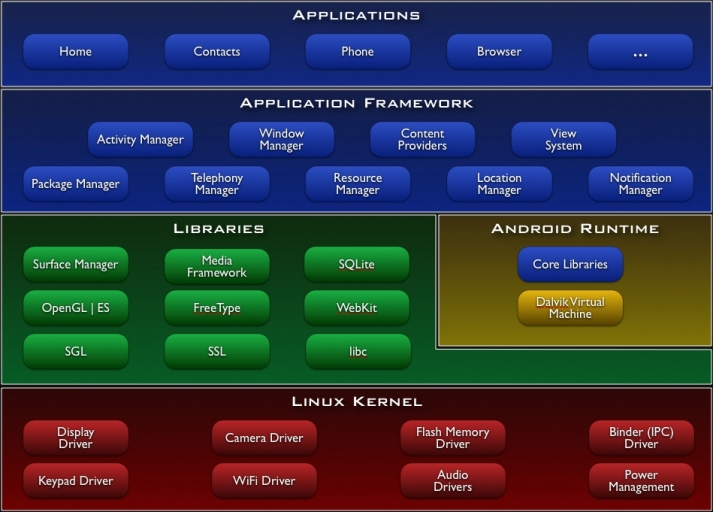
\includegraphics[width=\textwidth]{slides/android-introduction-architecture/architecture.jpg}
  \end{center}
\end{frame}

\begin{frame}
  \frametitle{The Linux Kernel}
  \begin{itemize}
  \item Used as the foundation of the Android system
  \item Numerous additions from the stock Linux, including new IPC (Inter-Process Communication) mechanisms,
    alternative power management mechanism, new drivers and various
    additions across the kernel
  \item These changes are beginning to go into the \path{staging/}
    area of the kernel, as of 3.3, after being a complete fork for a
    long time
  \end{itemize}
\end{frame}

\begin{frame}
  \frametitle{Android Libraries}
  \begin{itemize}
  \item Gather a lot of Android-specific libraries to interact at a
    low-level with the system, but third-parties libraries as well
  \item Bionic is the C library, SurfaceManager is used for drawing
    surfaces on the screen, etc.
  \item But also WebKit, SQLite, OpenSSL coming from the free software
    world
  \end{itemize}
\end{frame}

\begin{frame}
  \frametitle{Android Runtime}
  Handles the execution of Android applications
  \begin{itemize}
  \item Almost entirely written from scratch by Google
  \item Contains Dalvik, the virtual machine that executes every
    application that you run on Android, and the core library for the
    Java runtime, coming from Apache Harmony project
  \item Also contains system daemons, init executable, basic binaries,
    etc.
  \end{itemize}
\end{frame}

\begin{frame}
  \frametitle{Android Framework}
  \begin{itemize}
  \item Provides an API for developers to create applications
  \item Exposes all the needed subsystems by providing an abstraction
  \item Allows to easily use databases, create services, expose data
    to other applications, receive system events, etc.
  \end{itemize}
\end{frame}

\begin{frame}
  \frametitle{Android Applications}
  \begin{itemize}
  \item AOSP also comes with a set of applications such as the phone
    application, a browser, a contact management application, an email
    client, etc.
  \item However, the Google apps and the Android Market app aren't free
    software, so they are not available in AOSP. To obtain them, you
    must contact Google and pass a compatibility test.
  \end{itemize}
\end{frame}
